\documentclass[11pt, a4paper]{article}
\usepackage{graphicx}
\usepackage{amsmath}
\usepackage{listings}
\usepackage{color}
\usepackage{fancyhdr}
\usepackage[utf8]{inputenc}
\usepackage[%  
    colorlinks=true,
    pdfborder={0 0 0},
    linkcolor=red
]{hyperref}

\definecolor{dkgreen}{rgb}{0,0.6,0}
\definecolor{gray}{rgb}{0.5,0.5,0.5}
\definecolor{mauve}{rgb}{0.58,0,0.82}

\lstset{frame=tb,
  language=Python,
  aboveskip=3mm,
  belowskip=3mm,
  showstringspaces=false,
  columns=flexible,
  basicstyle={\small\ttfamily},
  numbers=none,
  numberstyle=\tiny\color{gray},
  keywordstyle=\color{blue},
  commentstyle=\color{dkgreen},
  stringstyle=\color{mauve},
  breaklines=true,
  breakatwhitespace=true,
  tabsize=3
}



\title{EE2703-Assignment6}
\author{EE19B094}
\date{April 2021}

\setlength{\headheight}{15pt}
\pagestyle{fancy}
\fancyhf{}
\rhead{Assignment - 6}
\lhead{EE2703 - Applied Programming Lab}
\rfoot{Page \thepage}

\begin{document}

\maketitle
\newpage

\begin{abstract}
    In this assignment, we model a tubelight in which electrons are continually injected at the cathode and accelerated towards the anode by a constant electric field. Electrons with velocity greater than a threshold can ionize atoms, which will released a photon. The tubelight is simulated for a certain number of timesteps. We look at effects of varying parameters.
\end{abstract}

\section{Simulation code}
We inject electrons into the tubelight following a normal distribution of mean $M$ and variance $Msig$, this electrons are accelerated through the tubelight and if the velocity of a particular electron is greater than a threshold then, it can collide and cause ionization. Thus, there are two main cases\\\\
Thus, in case of no collision the displacement of electron and velocity after one time stamp
\[
dx = u_i + 0.5
\]
\[
x_{i+1} = x_i + dx
\]
\[
u_{i+1} = u_i + 1
\]\\

Now, for finding electrons which collide, we first find the electrons with velocity greater than threshold and from them select electrons with given probability which take part in collision. Thus the position of those electrons after one time stamp,
\[
x_{i+1} = x_i + \rho dx
\]
where $\rho$ is a random number between 0 and 1 and $dx$ is the value calculated above. Thus selecting a random distance between $x_i$ and $x_i + dx$. Also, the velocity of the electron becomes zero i.e. $$u_{i+1} = 0$$ Note that here we haven't taken into account the increase in velocity in the remaining time in the time stamp after the collision, this error will be corrected later.

\begin{lstlisting}
#Taking inputs from sys.argv if given, if not give use the default values
try:
    if(len(sys.argv)==8):
        M=int(sys.argv[1])
        n=int(sys.argv[2])
        nk=int(sys.argv[3])  
        u0=float(sys.argv[4])
        p=float(sys.argv[5])
        Msig=float(sys.argv[6])
        accurate=int(sys.argv[7])
    else:
        print("Invalid format of parameters given in commandline")
        M = 5               #Number of electrons injected per turn.
        n=100               #Spatial grid size.
        nk=500              #Number of turns to simulate.
        u0=5                #Threshold velocity.
        p=0.25              #Probability that ionization will occur
        Msig=1              #Taking sigma of normal distribution = 1
        accurate = 1        #Whether to make more accurate calculations
except:
    print("Invalid format of parameters given in commandline")
    M = 5                   #Number of electrons injected per turn.
    n=100                   #Spatial grid size.
    nk=500                  #Number of turns to simulate.
    u0=5                    #Threshold velocity.
    p=0.25                  #Probability that ionization will occur
    Msig=1                  #Taking sigma of normal distribution = 1
    accurate = 1            #Whether to make more accurate calculations

xx = np.zeros(n*M)      #Electron position
u = np.zeros(n*M)       #Electron velocity  
dx = np.zeros(n*M)      #Electron displacement per time step

I = []          #Stores value of intensity of emitted light at every time-step
V = []          #Stores value of electron velocity at every time-step
X = []          #Stores value of electron position at every time-step    


#Carrying the iterations
for i in range(1,nk):
    ii = np.where(xx>0)[0]      #Electrons currently inside the tubelight
    
    dx[ii] = u[ii] + 0.5        #Displacement of electron with velocity u[ii]
    xx[ii] = xx[ii] + dx[ii]    #New position of electron
    u[ii] = u[ii] + 1.0         #New velocity of electron
    
    npos = np.where(xx>n)[0]    #Finding electrons which left the tubelight
    xx[npos] = 0.0              #Equate their parameters values to initial values
    dx[npos] = 0.0
    u[npos] = 0.0
    
    kk=np.where(u>=u0)[0]               #Incides of electrons capable of collision
    ll=np.where(rand(len(kk))<=p)[0]    #Chosing random electrons with probability p
    kl=kk[ll]                           #Indices of electrons undergone collision
    
    if accurate == 0:   #Less accurate calculations
        P = np.random.rand(len(kl))             #Choosing random 'position' between x_i and x_i+1
        xx[kl] = xx[kl]-np.multiply(dx[kl],P)   #and equating that as the position of collision
        u[kl] = 0                               #Also, velocity = 0 as collision is inelastic

    else:               #More accurate calculations
        dt = rand(len(kl))                              #Choosing random 'time' between 0 and 1
        xx[kl]=xx[kl]-dx[kl]+((u[kl]-1)*dt+0.5*dt*dt)   #Corresponding position of collision
        u[kl]=0                                         #Velocity = 0 after collision

        u[kl]+=1-dt                                     #Velocity of electron gained after collison
        xx[kl]+=0.5*(1-dt)**2                           #Distance travelled after collision

    
    I.extend(xx[kl].tolist())               #Increasing intensity at point of collision
    
    m=np.random.randn()*Msig+M              #Number of electrons inserted
    empty_xpos = np.where(xx==0)[0]         #Finding indices in position array to insert electrons
    electrons_generated = min(len(empty_xpos),(int)(m)) #If not enough space for all electrons, add as much as we can
    xx[empty_xpos[0:electrons_generated]] = 1.0
    u[empty_xpos[0:electrons_generated]] = 0.0
    
    X.extend(xx[ii].tolist())
    V.extend(u[ii].tolist())
\end{lstlisting}

\section{Plotting Graphs}
\begin{lstlisting}
class General_Plotter():
    ''' Class used for plotting different plots. Shortens the code by quite a bit'''
    
    def __init__(self,xlabel,ylabel,title,fig_num=0):
        ''' xlabel,ylabel,title are used in every graph''' 

        self.xlabel=xlabel
        self.ylabel=ylabel
        self.title=title
        self.fig=plt.figure(fig_num)
    
    def general_funcs(self,ax):
        ''' General functions for every graph'''
        
        ax.set_ylabel(self.ylabel)
        ax.set_xlabel(self.xlabel)
        ax.set_title(self.title)
        plt.show()
        #self.fig.savefig(self.title+".png")

    def population_plot(self,values):
        axes=self.fig.add_subplot(111)
        axes.hist(values,histtype='bar',ec='black',bins=100)
        self.general_funcs(axes)

    def scatter_plot(self,X,Y):
        axes=self.fig.add_subplot(111)
        a=list(zip(X, Y))
        a=set(a)
        X,Y=zip(*a)
        axes.scatter(X,Y,c='r',marker='x')
        self.general_funcs(axes)

# Plotting graphs

p1=General_Plotter("Grid_Space","Number of Electrons","Population_Plot_of_Electrons",0)
p1.population_plot(X)
p2=General_Plotter("Grid_Space","Intensity of Light","Intensity of Light",1)
p2.population_plot(I)
p3=General_Plotter("X","V","X vs V",2)
p3.scatter_plot(X,V)




# Tabulating data for intensity vs position
bins = plt.hist(I,bins=np.arange(1,n,n/100))[1]    # Bin positions are obtained
count = plt.hist(I,bins=np.arange(1,n,n/100))[0]   # Population counts obtained
xpos = 0.5*(bins[0:-1] + bins[1:])     # As no. of end-points of bins would be 1 more than actual no. of bins, the mean of bin end-points are used to get population of count a particular bin
df = pd.DataFrame()   # A pandas dataframe is initialized to do the tabular plotting of values.
df['Xpos'] = xpos
df['count'] = count

base_filename = 'values.txt'
with open(base_filename,'w') as outfile:
    df.to_string(outfile)
\end{lstlisting}

\section{Simulation for varying parameters and accuracy}
The list of parameters are,\\
M -- Number of electrons injected per turn.\\
n -- Spatial grid size.\\
nk -- Number of turns to simulate.\\
u0 -- Threshold velocity.\\
p -- Probability that ionization will occur\\               
Msig -- Taking sigma of normal distribution\\
accurate -- Whether to make more accurate calculations\\

\subsection{Parameter set 1}
For, the parameters value M=5 , n=100, nk=500, u0=7, p=0.25, Msig=1, accurate=0, the graphs are
\begin{figure}[!tbh]
    \centering
    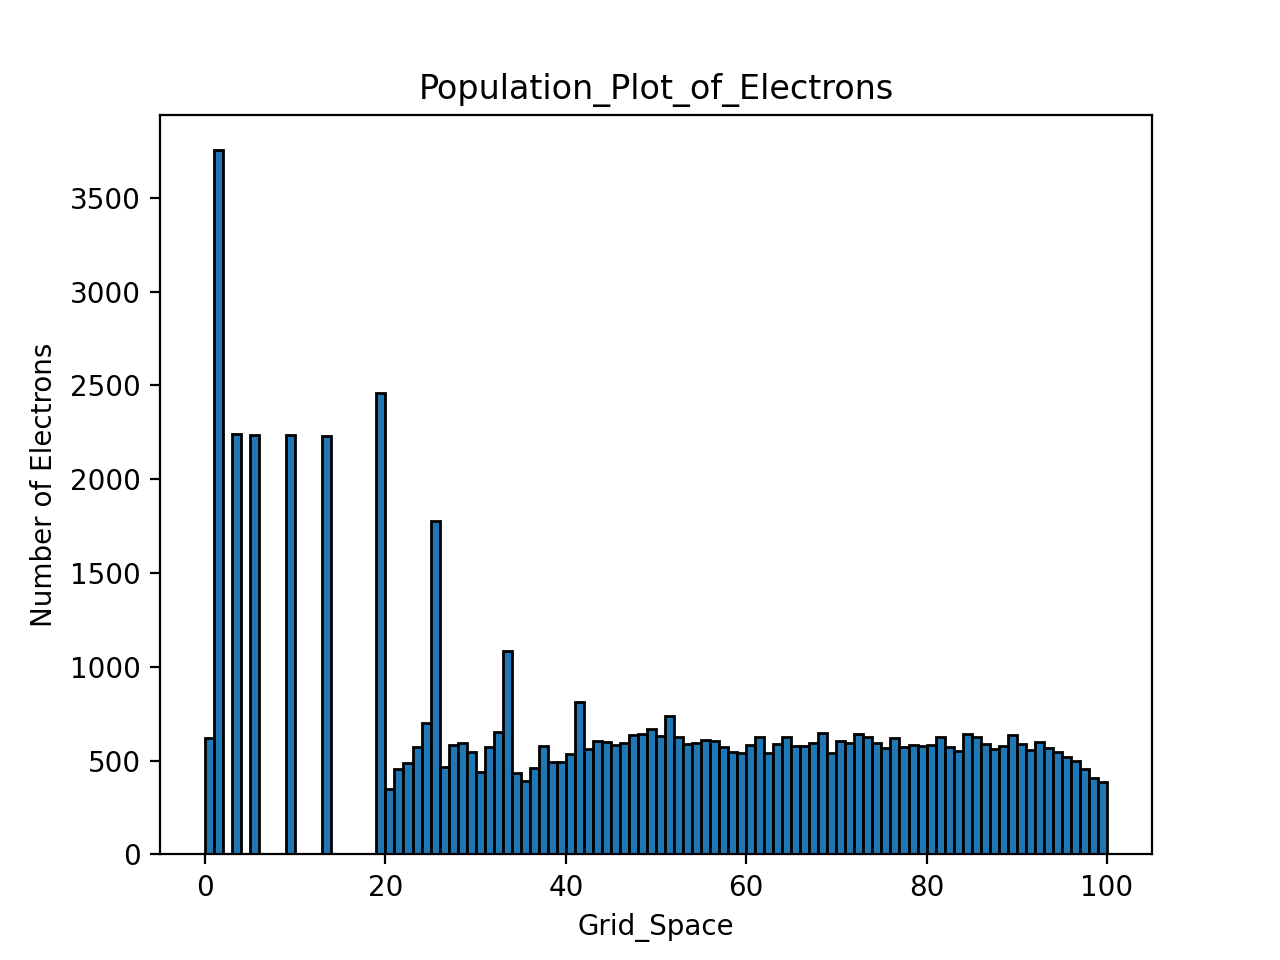
\includegraphics[scale = 0.7]{default_1.png}
\end{figure}
\begin{figure}[!tbh]
    \centering
    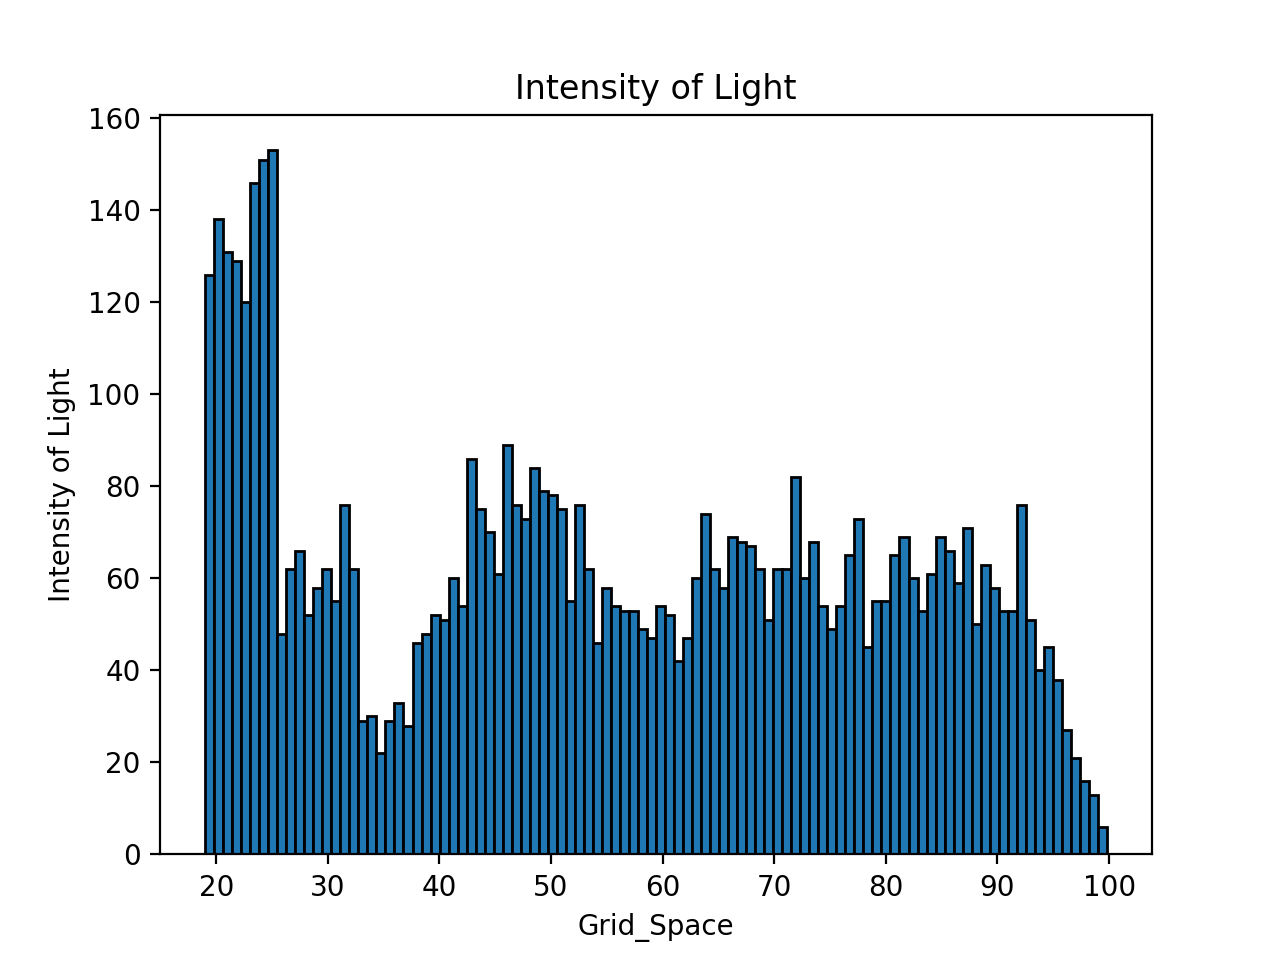
\includegraphics[scale = 0.7]{default_2.png}
\end{figure}
\begin{figure}[!tbh]
    \centering
    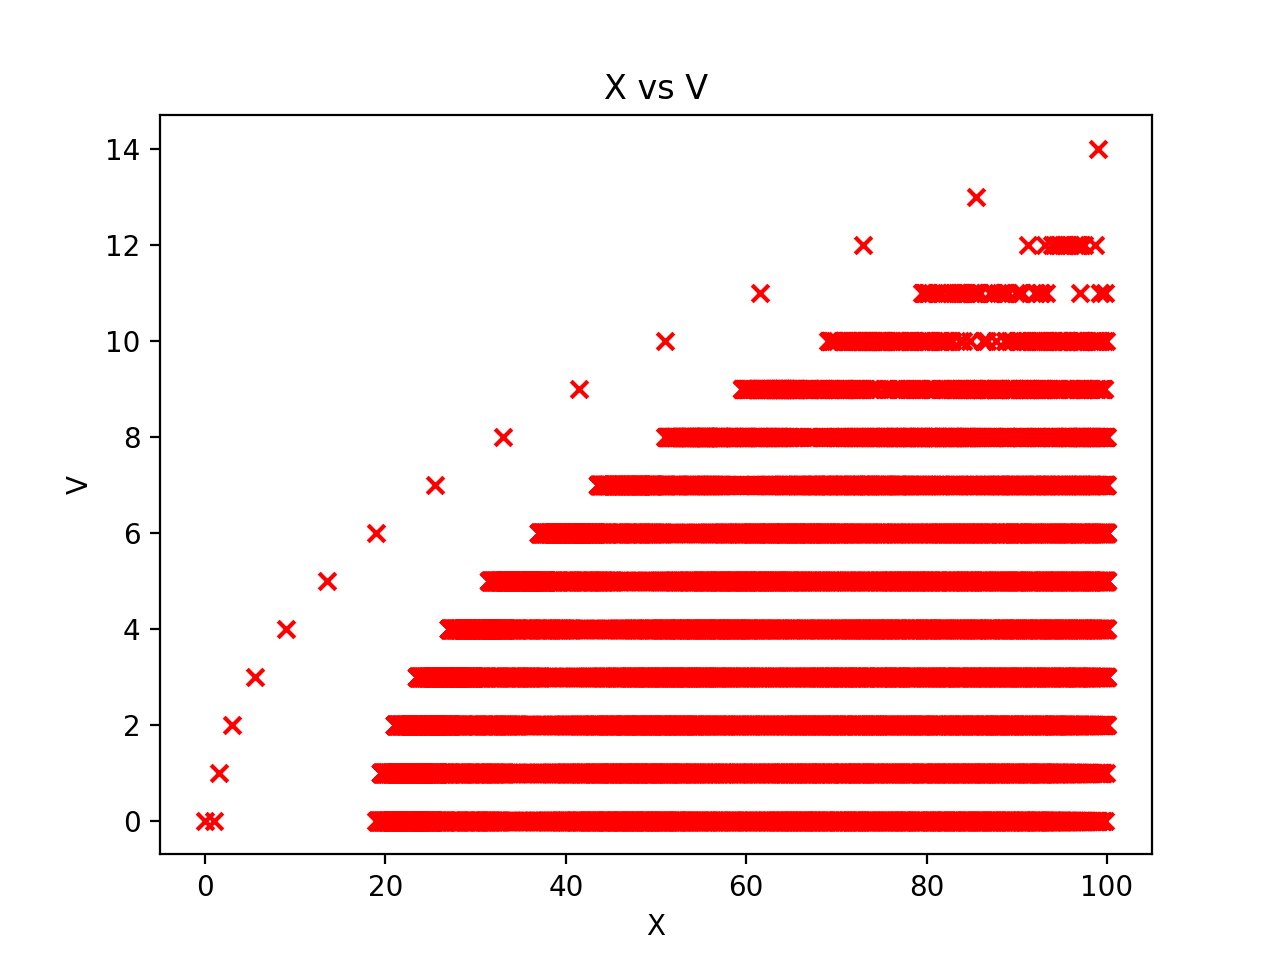
\includegraphics[scale = 0.7]{default_3.png}
\end{figure}

\newpage
\subsubsection{Observations}
  As, initially the electrons start out with 0 velocity, at small values of position they are slow and thus no chances of collision, and thus we see that the electron density has peaks in the beginning.\\

  Now around x = 19, the electrons reach the threshold velocity of u0 = 7, and thus collisions occur, which can be seen from peaks near x = 19 in the Intensity plot.\\

  While from the phase plot, we can see that the sets of points corresponding to \(v \space = k \sqrt{x}\) are seperated from the rest of the curve. This corresponds to the electrons which suffer no collisions throughtout. Also, as in our calculations, we do not accelerate the electron again after the collision for that timestamp, the velocities are discrete in nature.\\

\subsection{Parameter set 2}
Now, if we make more accurate corrections by randomly choosing \emph{time} for collision and also, we accelerate the electrons for the rest of the time in that time-stamp i.e.\\
Suppose the time of collision is $t$, then the total distance covered by the electron will be, 
\[
dx = \underbrace{u_i + \frac{1}{2}t^2}_\text{Below collision} + \overbrace{\frac{1}{2}(1-t)^2}^\text{After collision}
\]\\
and the velocity will be,
\[
u_{i+1} = 1 - t
\]\\
Now, the graphs change as follows,

\begin{figure}[!tbh]
    \centering
    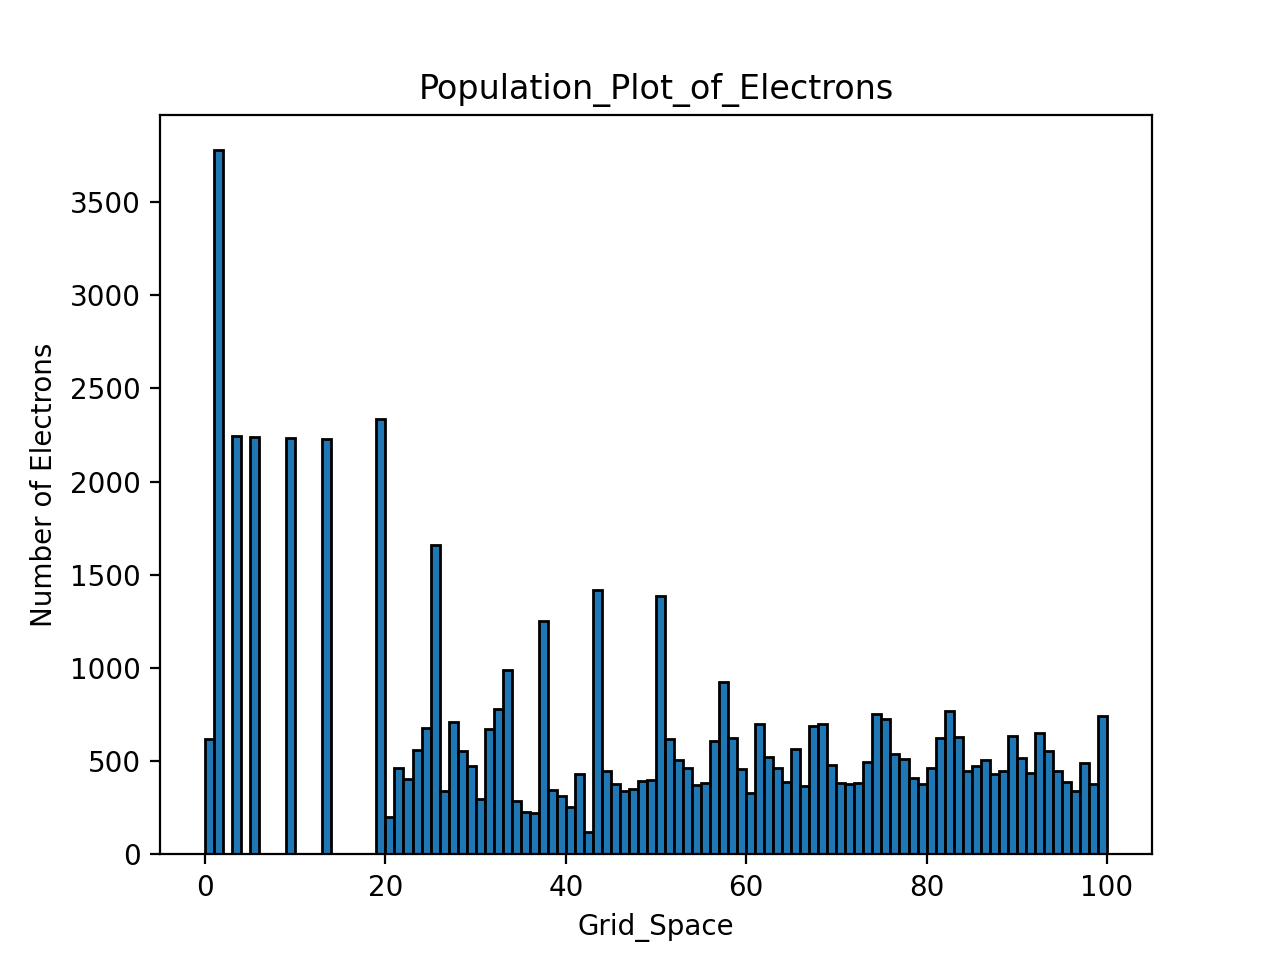
\includegraphics[scale = 0.7]{default_1_1.png}
\end{figure}
\begin{figure}[!tbh]
    \centering
    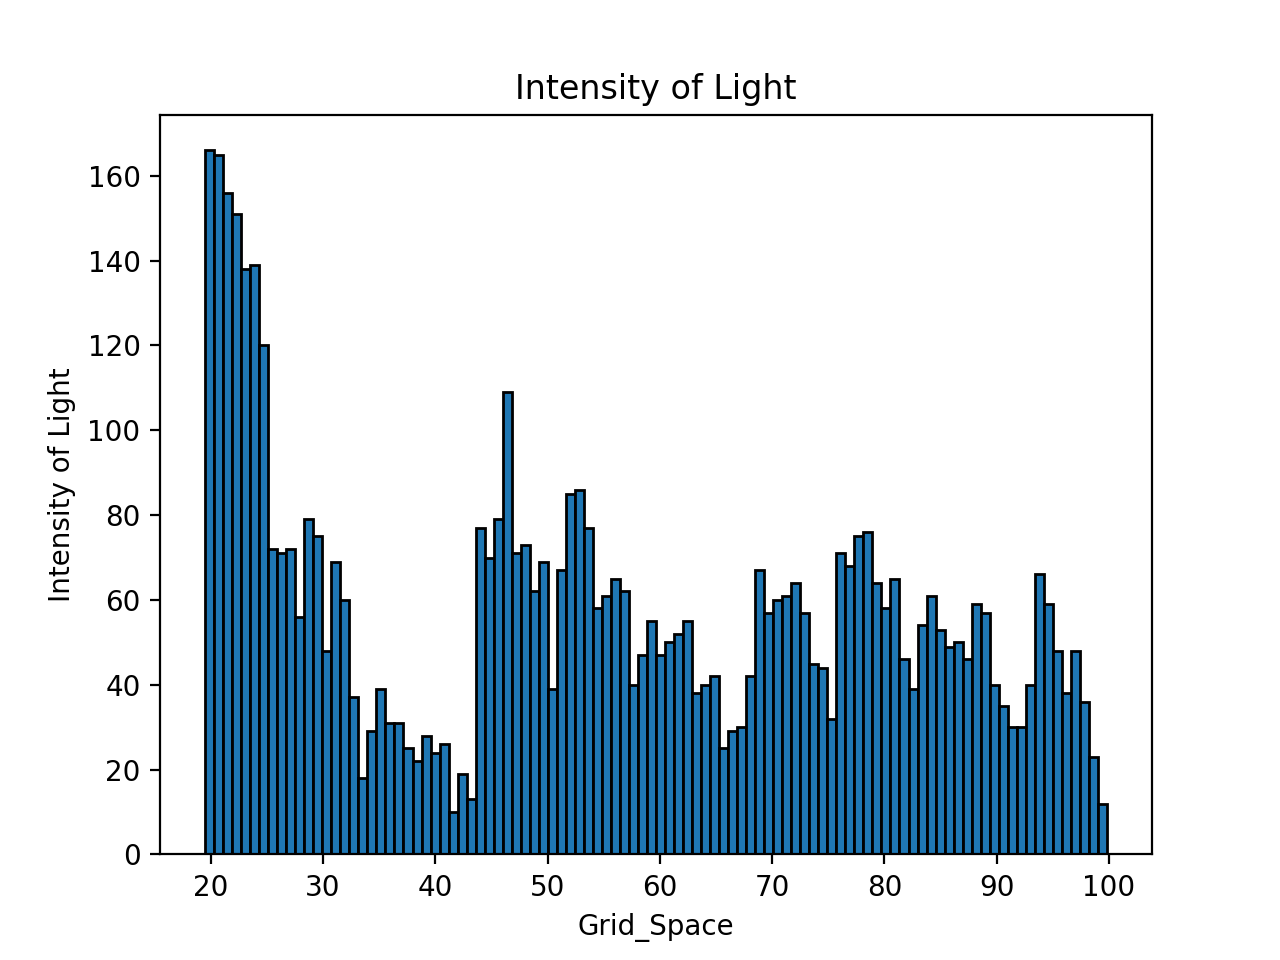
\includegraphics[scale = 0.7]{default_2_1.png}
\end{figure}
\begin{figure}[!tbh]
    \centering
    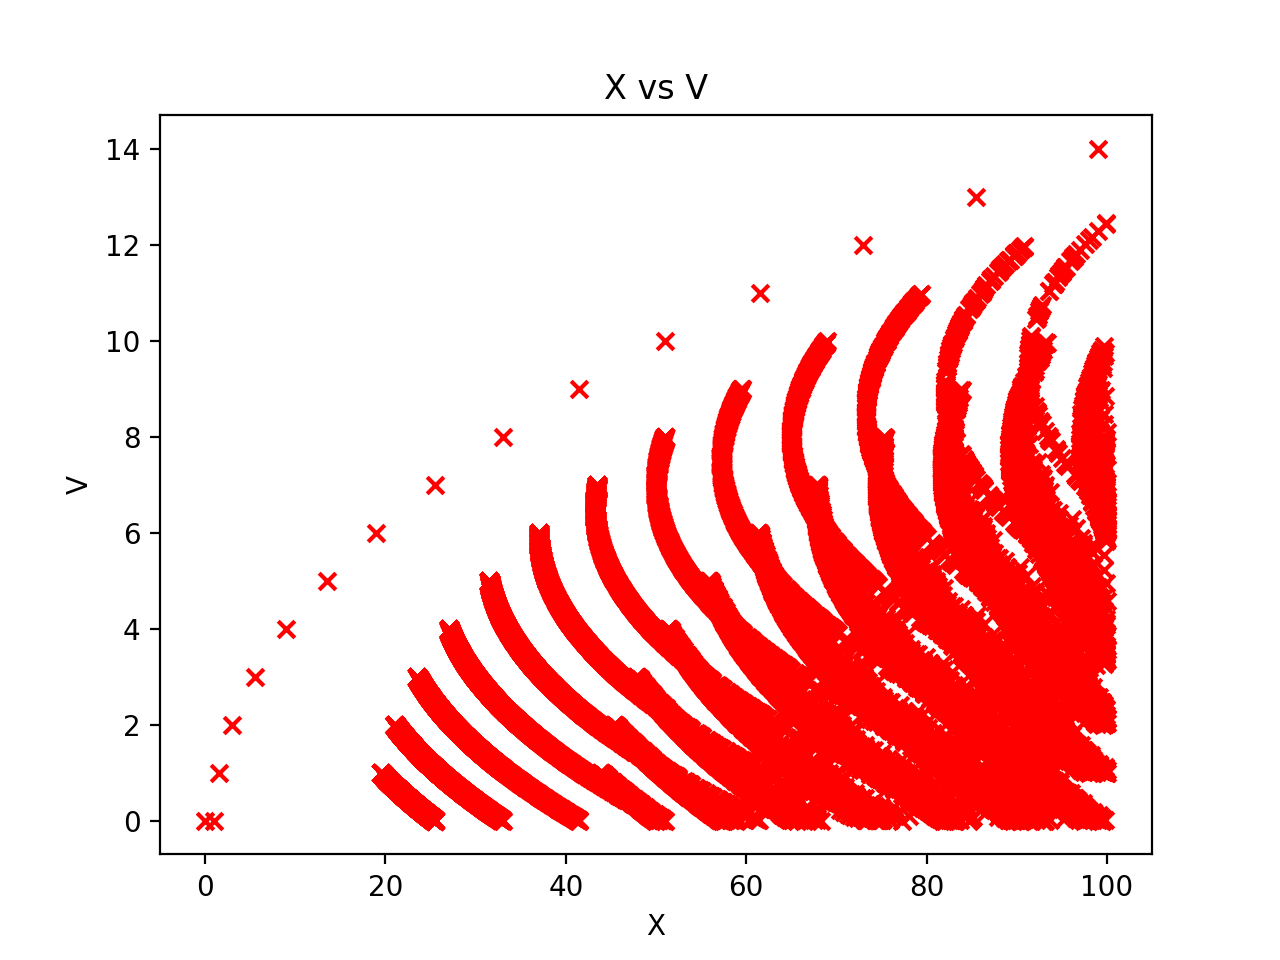
\includegraphics[scale = 0.7]{default_3_1.png}
\end{figure}\newpage

We can see here now that the velocities are continuous in nature.\\\\
The count at various positions of x are,
\begin{verbatim}
        Xpos  count
0    1.5    0.0
1    2.5    0.0
2    3.5    0.0
3    4.5    0.0
4    5.5    0.0
5    6.5    0.0
6    7.5    0.0
7    8.5    0.0
8    9.5    0.0
9   10.5    0.0
10  11.5    0.0
11  12.5    0.0
12  13.5    0.0
13  14.5    0.0
14  15.5    0.0
15  16.5    0.0
16  17.5    0.0
17  18.5    0.0
18  19.5  108.0
19  20.5  199.0
20  21.5  200.0
21  22.5  172.0
22  23.5  184.0
23  24.5  156.0
24  25.5   88.0
25  26.5   96.0
26  27.5   86.0
27  28.5   88.0
28  29.5   86.0
29  30.5   65.0
30  31.5   79.0
31  32.5   67.0
32  33.5   19.0
33  34.5   43.0
34  35.5   41.0
35  36.5   38.0
36  37.5   33.0
37  38.5   26.0
38  39.5   40.0
39  40.5   26.0
40  41.5   17.0
41  42.5   22.0
42  43.5   36.0
43  44.5  101.0
44  45.5   99.0
45  46.5  120.0
46  47.5   93.0
47  48.5   84.0
48  49.5   85.0
49  50.5   54.0
50  51.5   89.0
51  52.5  104.0
52  53.5  108.0
53  54.5   77.0
54  55.5   67.0
55  56.5   85.0
56  57.5   56.0
57  58.5   63.0
58  59.5   63.0
59  60.5   62.0
60  61.5   58.0
61  62.5   71.0
62  63.5   45.0
63  64.5   55.0
64  65.5   34.0
65  66.5   38.0
66  67.5   40.0
67  68.5   68.0
68  69.5   72.0
69  70.5   82.0
70  71.5   78.0
71  72.5   73.0
72  73.5   56.0
73  74.5   54.0
74  75.5   54.0
75  76.5   84.0
76  77.5   91.0
77  78.5   93.0
78  79.5   75.0
79  80.5   88.0
80  81.5   60.0
81  82.5   47.0
82  83.5   61.0
83  84.5   84.0
84  85.5   63.0
85  86.5   61.0
86  87.5   60.0
87  88.5   68.0
88  89.5   61.0
89  90.5   46.0
90  91.5   36.0
91  92.5   45.0
92  93.5   72.0
93  94.5   71.0
94  95.5   57.0
95  96.5   56.0
96  97.5   52.0
97  98.5   28.0
\end{verbatim}

\newpage
\subsection{Parameter set 3}
Now, let's say we decrease the threshold velocity to low value u0=2.5, and increase the probability of collision p=0.95, then the plots become

\begin{figure}[!tbh]
    \centering
    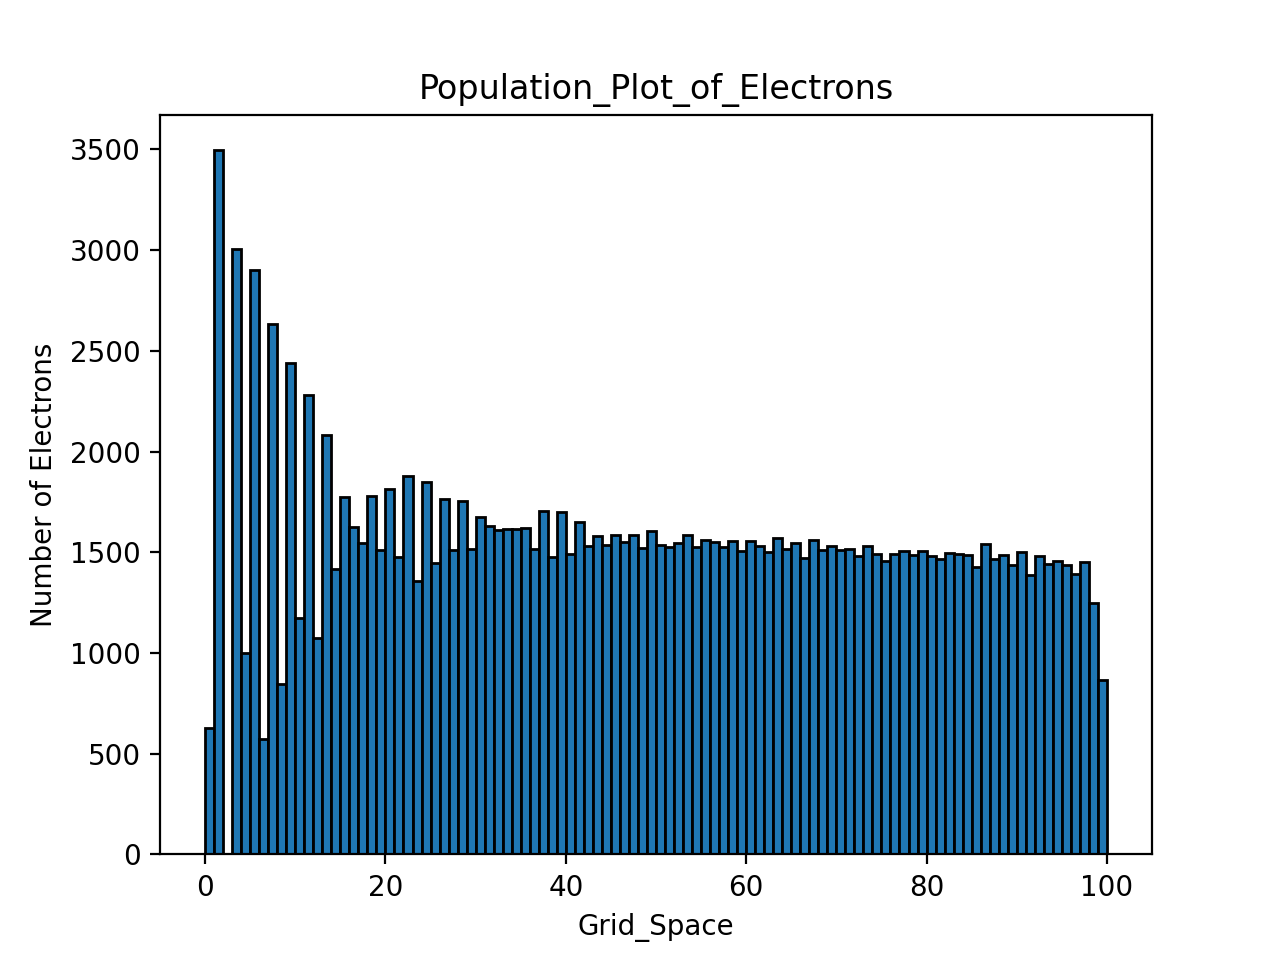
\includegraphics[scale = 0.7]{set3_1.png}
\end{figure}
\begin{figure}[!tbh]
    \centering
    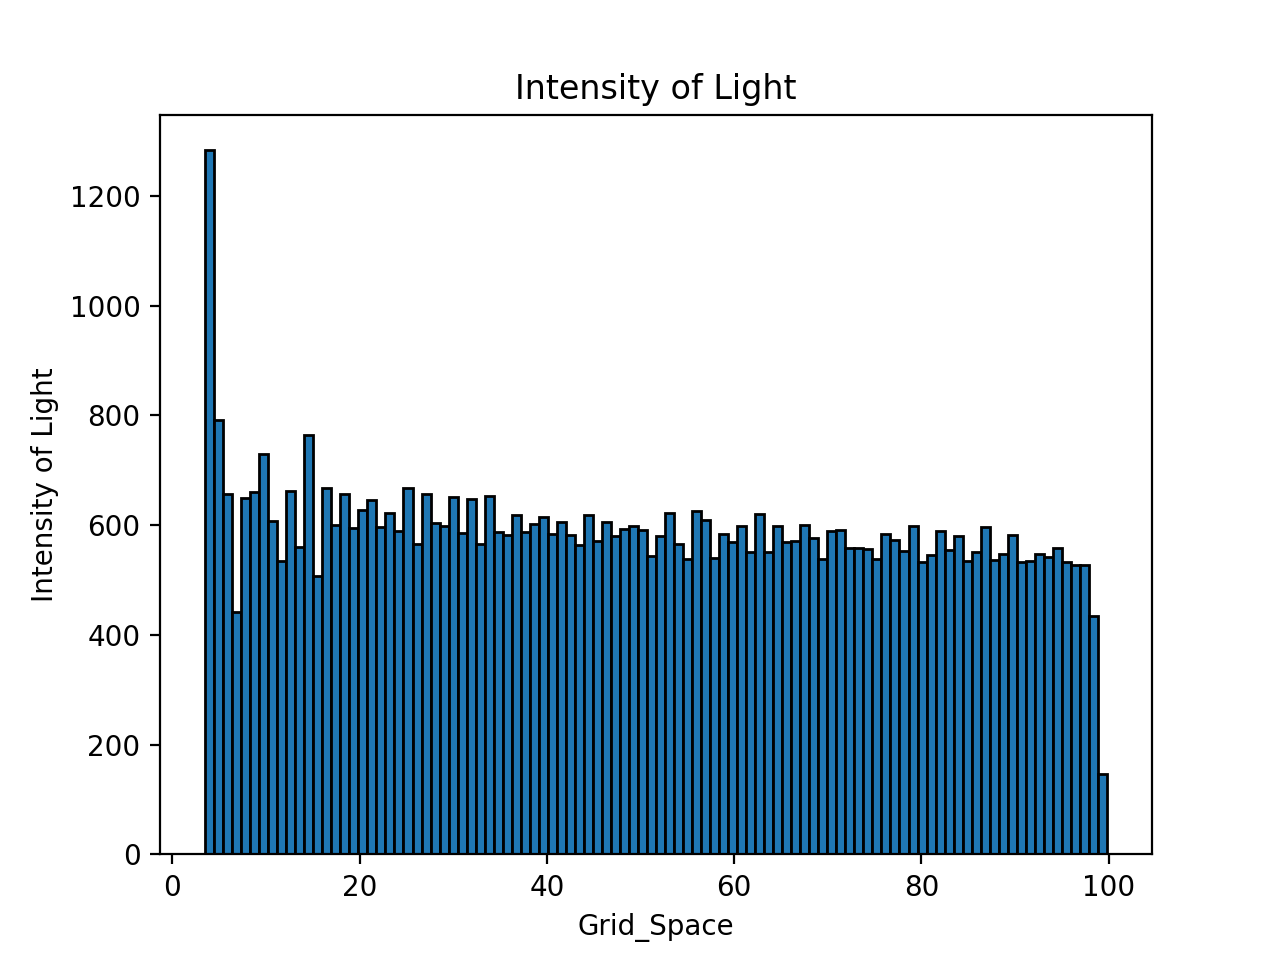
\includegraphics[scale = 0.7]{set3_2.png}
\end{figure}
\begin{figure}[!tbh]
    \centering
    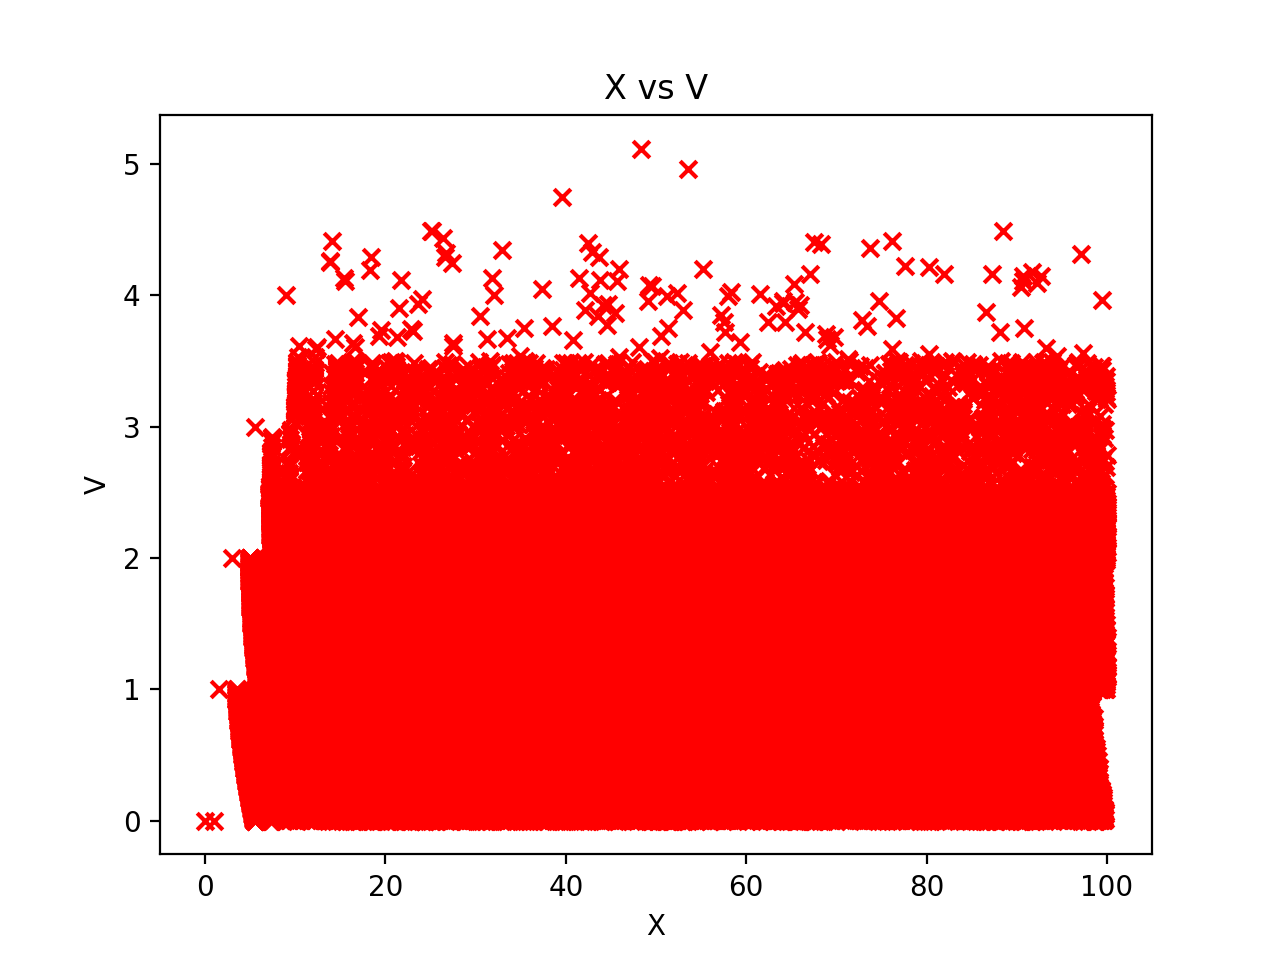
\includegraphics[scale = 0.7]{set3_3.png}
\end{figure}


\section{Conclusion}
From parameter set 3 we can see that, as the threshold is very low, thus the intensity starts from low values of x. Also, as electrons gain threshold velocity after around 3 timestamps, the intensity curve is smooth and the electron density curve is uniform.\\

Also due to high probability of collision, more number of electrons will collide and thus the total intensity of light will be more.\\

Thus, in general, we would prefer tublights filled with gas whose threshold is low and probability of collision is high, as this gives us uniform and high intensity.
\end{document}
